% This figure is Hopfield dynamics.
\RequirePackage{luatex85,shellesc}
\documentclass[crop,multi=false]{standalone}
\usepackage{tabularx}
\usepackage{pgfplots}

% \usepackage[sfdefault]{FiraSans}
% \usepackage[small]{eulervm}
\usepackage{opensans}
\usepackage{mathpazo}

% Based on http://www.texample.net/tikz/examples/neural-network/
\usepackage{tikz}
\usetikzlibrary{arrows,arrows.meta,calc,positioning}
\def\layersep{2.5cm}

% colwidth in cm
\edef\ColWidth{5}

\begin{document}

\newcommand\PlotLetter[2]{ % filename, title 
    \edef\Width{15}
    \begin{tikzpicture}[ ]
        \begin{axis}[ 
            view={0}{90}
            , width = \Width  mm, height = \Width mm, scale only axis
            , xtick=\empty, ytick=\empty
            % , colormap name={viridis}
            , colormap={jet}{samples of colormap=(2)}
            , title={#2}
            , title style={font=\footnotesize, at={(0.5,1)}, anchor=south
                , align=left
                }
            ]
            \addplot[matrix plot*, mesh/cols=10] table [
                x index=1
                , y expr=10-\thisrowno{0}
                , point meta=\thisrowno{2}
                ] {#1};
        \end{axis}
    \end{tikzpicture}	
}

\begin{tikzpicture}
    \node[ ] (a) {
        \begin{tikzpicture}[baseline, scale=1 , every node/.style={} ]
            \edef\CLR{blue}

            \node[circle, inner sep=4mm, fill=\CLR!20
                , label={[yshift=5mm]above:{\footnotesize if $I+\sum_i w_i i_i >
                    0$ then 1 else -1}}
                ] (nrn) {};

            \node[above=of nrn] (title) {Simplified Neuron};

            % draw synapse
            \foreach \i/\theta in {1/-15,2/-30,3/-45}
            {
                \pgfmathsetmacro\ang{0.5*\theta}
                \node[inner sep=2pt, circle, fill=\CLR, shift=(\theta:-7mm)] (syn\i) {};
                \node[right=of syn\i, xshift=-10mm] {\tiny $w_\i$};
                \draw[-, draw=\CLR] (syn\i) -- ++(\ang:-5mm) node[left] {\tiny $i_\i$};
            }
            \draw[thick, -*] (nrn) -- ++(2,0);
            \draw[thick, *-] (nrn) -- ++(-1.5,0) node[left] {I};
        \end{tikzpicture}
    };
    \node[above left=1mm of a] (alabel) {\bf A};

    \node[below=10mm of a.south west, anchor=north west
        , label={above:Hopfield Network}
        ] (b) {

        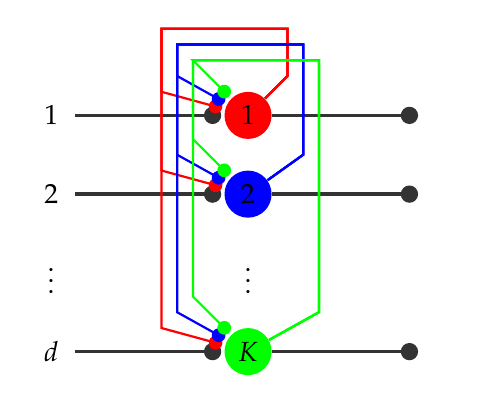
\begin{tikzpicture}[baseline, shorten >=1pt, -Circle, draw=black!80, node distance=\layersep]
            \tikzstyle{every pin edge}=[<-,shorten <=1pt]
            \tikzstyle{neuron}=[circle, minimum size=17pt,inner sep=0pt]
            \tikzstyle{phantomneuron}=[circle,fill=black!0,minimum size=17pt,inner sep=0pt]
            \tikzstyle{annot} = [text width=4em, text centered]

            % Draw the input layer nodes
            \foreach \name / \y in {1/1,2/2,$d$/4}
                \node[phantomneuron] (I-\y) at (0,-\y) {\name};
            \node (I-3) at (0,-3) {\vdots};

            % Draw the hidden layer nodes
            \foreach \name/\y/\color in {1/1/red,2/2/blue,$K$/4/green}
                \node[neuron, fill=\color, minimum width=5mm] (H-\y) at (\layersep,-\y) {\name};
            \node (H-3) at (\layersep,-3) {\vdots};

            \foreach \name / \y in {1/1,2/2,$d$/4}
               \node[phantomneuron] (O-\y) at (2*\layersep,-\y) {};

            % Connect every node in the input layer with every node in the
            % hidden layer.
            \foreach \source in {1,2,4}
                    \path[very thick] (I-\source) edge (H-\source);
           
            % Connect every node in the hidden layer with the output layer
            \foreach \source in {1,2,4}
                    \path[very thick] (H-\source) edge (O-\source);
                    
            \foreach \dest / \y in {1/1, 2/2, $d$/4}
                \draw[thick,color=red] (H-1) -- + (0.5, 0.5) -- + (0.5, 1.1) --+ (-1.1, 1.1) -- + (-1.1, -\y+1.3) -- + (H-\y);

            \foreach \dest / \y in {1/1, 2/2, $d$/4}
                \draw[thick,color=blue] (H-2) -- + (0.7, 0.5) -- + (0.7, 1.9) -- + (-0.9, 1.9) -- + (-0.9, -\y+2.5) -- + (H-\y);

            \foreach \dest / \y in {1/1, 2/2, $d$/4}
                \draw[thick,color=green] (H-4) -- + (0.9, 0.5) -- + (0.9,3.7) -- + (-0.7, 3.7) -- + (-0.7, -\y+4.7) -- + (H-\y);

        \end{tikzpicture} 
    };

    \node[right=of a.north east, anchor=north west, text width=\ColWidth cm] (stored) {
        Stored Patterns  \\

        \begin{tabular}{c c c}
        \PlotLetter{../hopfield/N.txt}{} & \PlotLetter{../hopfield/C.txt}{} & \PlotLetter{../hopfield/B.txt}{} \\
        \PlotLetter{../hopfield/S.txt}{} & \PlotLetter{../hopfield/X.txt}{} & \PlotLetter{../hopfield/Y.txt}{} \\
        \end{tabular}
    };
    \node[above left=1mm of stored] (labelB) {\textbf{B}};

    \node[below=5mm of stored.south west, anchor=north west] (fetchB) {
        \begin{tabular}{l l l}
        \PlotLetter{../hopfield/B0.txt}{Input cue\\ B+50\% noise} &
            \PlotLetter{../hopfield/B1.txt}{Recall\\after 1 step} &
            \PlotLetter{../hopfield/B2.txt}{Recall\\after 2 steps} \\
        \PlotLetter{../hopfield/X0.txt}{Input cue\\ X+50\% noise} &
            \PlotLetter{../hopfield/X1.txt}{Recall\\after 1 step} & 
            \PlotLetter{../hopfield/X2.txt}{Recall\\after 2 steps}
        \end{tabular}
    };
    \node[above left=-1mm of fetchB] (labelC) {\textbf{C}};

\end{tikzpicture}
\end{document}

